\documentclass[twoside]{book}

% Packages required by doxygen
\usepackage{fixltx2e}
\usepackage{calc}
\usepackage{doxygen}
\usepackage[export]{adjustbox} % also loads graphicx
\usepackage{graphicx}
\usepackage[utf8]{inputenc}
\usepackage{makeidx}
\usepackage{multicol}
\usepackage{multirow}
\PassOptionsToPackage{warn}{textcomp}
\usepackage{textcomp}
\usepackage[nointegrals]{wasysym}
\usepackage[table]{xcolor}

% NLS support packages
\usepackage[catalan]{babel}

% Font selection
\usepackage[T1]{fontenc}
\usepackage[scaled=.90]{helvet}
\usepackage{courier}
\usepackage{amssymb}
\usepackage{sectsty}
\renewcommand{\familydefault}{\sfdefault}
\allsectionsfont{%
  \fontseries{bc}\selectfont%
  \color{darkgray}%
}
\renewcommand{\DoxyLabelFont}{%
  \fontseries{bc}\selectfont%
  \color{darkgray}%
}
\newcommand{\+}{\discretionary{\mbox{\scriptsize$\hookleftarrow$}}{}{}}

% Page & text layout
\usepackage{geometry}
\geometry{%
  a4paper,%
  top=2.5cm,%
  bottom=2.5cm,%
  left=2.5cm,%
  right=2.5cm%
}
\tolerance=750
\hfuzz=15pt
\hbadness=750
\setlength{\emergencystretch}{15pt}
\setlength{\parindent}{0cm}
\setlength{\parskip}{3ex plus 2ex minus 2ex}
\makeatletter
\renewcommand{\paragraph}{%
  \@startsection{paragraph}{4}{0ex}{-1.0ex}{1.0ex}{%
    \normalfont\normalsize\bfseries\SS@parafont%
  }%
}
\renewcommand{\subparagraph}{%
  \@startsection{subparagraph}{5}{0ex}{-1.0ex}{1.0ex}{%
    \normalfont\normalsize\bfseries\SS@subparafont%
  }%
}
\makeatother

% Headers & footers
\usepackage{fancyhdr}
\pagestyle{fancyplain}
\fancyhead[LE]{\fancyplain{}{\bfseries\thepage}}
\fancyhead[CE]{\fancyplain{}{}}
\fancyhead[RE]{\fancyplain{}{\bfseries\leftmark}}
\fancyhead[LO]{\fancyplain{}{\bfseries\rightmark}}
\fancyhead[CO]{\fancyplain{}{}}
\fancyhead[RO]{\fancyplain{}{\bfseries\thepage}}
\fancyfoot[LE]{\fancyplain{}{}}
\fancyfoot[CE]{\fancyplain{}{}}
\fancyfoot[RE]{\fancyplain{}{\bfseries\scriptsize Generat per Doxygen }}
\fancyfoot[LO]{\fancyplain{}{\bfseries\scriptsize Generat per Doxygen }}
\fancyfoot[CO]{\fancyplain{}{}}
\fancyfoot[RO]{\fancyplain{}{}}
\renewcommand{\footrulewidth}{0.4pt}
\renewcommand{\chaptermark}[1]{%
  \markboth{#1}{}%
}
\renewcommand{\sectionmark}[1]{%
  \markright{\thesection\ #1}%
}

% Indices & bibliography
\usepackage{natbib}
\usepackage[titles]{tocloft}
\setcounter{tocdepth}{3}
\setcounter{secnumdepth}{5}
\makeindex

% Hyperlinks (required, but should be loaded last)
\usepackage{ifpdf}
\ifpdf
  \usepackage[pdftex,pagebackref=true]{hyperref}
\else
  \usepackage[ps2pdf,pagebackref=true]{hyperref}
\fi
\hypersetup{%
  colorlinks=true,%
  linkcolor=blue,%
  citecolor=blue,%
  unicode%
}

% Custom commands
\newcommand{\clearemptydoublepage}{%
  \newpage{\pagestyle{empty}\cleardoublepage}%
}

\usepackage{caption}
\captionsetup{labelsep=space,justification=centering,font={bf},singlelinecheck=off,skip=4pt,position=top}

%===== C O N T E N T S =====

\begin{document}

% Titlepage & ToC
\hypersetup{pageanchor=false,
             bookmarksnumbered=true,
             pdfencoding=unicode
            }
\pagenumbering{roman}
\begin{titlepage}
\vspace*{7cm}
\begin{center}%
{\Large Pràctica P\+R\+O2 victor.\+sanchez.\+gassull \\[1ex]\large versió def 14-\/des-\/2017 }\\
\vspace*{1cm}
{\large Generat per Doxygen 1.8.11}\\
\end{center}
\end{titlepage}
\clearemptydoublepage
\tableofcontents
\clearemptydoublepage
\pagenumbering{arabic}
\hypersetup{pageanchor=true}

%--- Begin generated contents ---
\chapter{Índex de Classes}
\section{Llista de Classes}
Aquestes són les classes, estructures, unions i interfícies acompanyades amb breus descripcions\+:\begin{DoxyCompactList}
\item\contentsline{section}{\hyperlink{class_bin_tree}{Bin\+Tree$<$ T $>$} }{\pageref{class_bin_tree}}{}
\item\contentsline{section}{\hyperlink{class_experiment}{Experiment} }{\pageref{class_experiment}}{}
\item\contentsline{section}{\hyperlink{class_familia__individus}{Familia\+\_\+individus} }{\pageref{class_familia__individus}}{}
\item\contentsline{section}{\hyperlink{class_individu}{Individu} }{\pageref{class_individu}}{}
\item\contentsline{section}{\hyperlink{class_parell__cromosomes}{Parell\+\_\+cromosomes} }{\pageref{class_parell__cromosomes}}{}
\item\contentsline{section}{\hyperlink{class_tret}{Tret} }{\pageref{class_tret}}{}
\end{DoxyCompactList}

\chapter{Índex de Fitxers}
\section{Llista dels Fitxers}
Aquesta és la llista de tots els fitxers acompanyats amb breus descripcions\+:\begin{DoxyCompactList}
\item\contentsline{section}{\hyperlink{_bin_tree_8hh}{Bin\+Tree.\+hh} }{\pageref{_bin_tree_8hh}}{}
\item\contentsline{section}{\hyperlink{_experiment_8hh}{Experiment.\+hh} }{\pageref{_experiment_8hh}}{}
\item\contentsline{section}{\hyperlink{_familia__individus_8hh}{Familia\+\_\+individus.\+hh} }{\pageref{_familia__individus_8hh}}{}
\item\contentsline{section}{\hyperlink{_individu_8hh}{Individu.\+hh} }{\pageref{_individu_8hh}}{}
\item\contentsline{section}{\hyperlink{_parell__cromosomes_8hh}{Parell\+\_\+cromosomes.\+hh} }{\pageref{_parell__cromosomes_8hh}}{}
\item\contentsline{section}{\hyperlink{_tret_8hh}{Tret.\+hh} }{\pageref{_tret_8hh}}{}
\end{DoxyCompactList}

\chapter{Documentació de les Classes}
\hypertarget{class_bin_tree}{}\section{Referència de la Classe Template Bin\+Tree$<$ T $>$}
\label{class_bin_tree}\index{Bin\+Tree$<$ T $>$@{Bin\+Tree$<$ T $>$}}
\subsection*{Mètodes públics}
\begin{DoxyCompactItemize}
\item 
\hyperlink{class_bin_tree_a47eef22d29cd023449d97c073c08e5b6}{Bin\+Tree} ()
\item 
\hyperlink{class_bin_tree_a1ab686e0bcf990093ff91fe71744c1a4}{Bin\+Tree} (const T \&x)
\item 
\hyperlink{class_bin_tree_adb7eeff76d08130c943b36af215eb521}{Bin\+Tree} (const T \&x, const \hyperlink{class_bin_tree}{Bin\+Tree} \&\hyperlink{class_bin_tree_a781025fb1c3693e91e851d55b181bedd}{left}, const \hyperlink{class_bin_tree}{Bin\+Tree} \&\hyperlink{class_bin_tree_a009c4bb95a25a1b639da637de32101ce}{right})
\item 
bool \hyperlink{class_bin_tree_a9ca8d7ae95b9bed51eb43f30c8d2bd58}{empty} () const 
\item 
\hyperlink{class_bin_tree}{Bin\+Tree} \hyperlink{class_bin_tree_a781025fb1c3693e91e851d55b181bedd}{left} () const 
\item 
\hyperlink{class_bin_tree}{Bin\+Tree} \hyperlink{class_bin_tree_a009c4bb95a25a1b639da637de32101ce}{right} () const 
\item 
const T \& \hyperlink{class_bin_tree_af545517333e94fdbfccfbc7df7d961fe}{value} () const 
\end{DoxyCompactItemize}


\subsection{Descripció Detallada}
\subsubsection*{template$<$typename T$>$\\*
class Bin\+Tree$<$ T $>$}



Definició a la línia 12 del fitxer Bin\+Tree.\+hh.



\subsection{Documentació del Constructor i el Destructor}
\index{Bin\+Tree@{Bin\+Tree}!Bin\+Tree@{Bin\+Tree}}
\index{Bin\+Tree@{Bin\+Tree}!Bin\+Tree@{Bin\+Tree}}
\subsubsection[{\texorpdfstring{Bin\+Tree()}{BinTree()}}]{\setlength{\rightskip}{0pt plus 5cm}template$<$typename T$>$ {\bf Bin\+Tree}$<$ T $>$\+::{\bf Bin\+Tree} (
\begin{DoxyParamCaption}
{}
\end{DoxyParamCaption}
)}\hypertarget{class_bin_tree_a47eef22d29cd023449d97c073c08e5b6}{}\label{class_bin_tree_a47eef22d29cd023449d97c073c08e5b6}


Definició a la línia 41 del fitxer Bin\+Tree.\+hh.


\begin{DoxyCode}
42     :   p(\textcolor{keyword}{nullptr})
43     \{   \}
\end{DoxyCode}
\index{Bin\+Tree@{Bin\+Tree}!Bin\+Tree@{Bin\+Tree}}
\index{Bin\+Tree@{Bin\+Tree}!Bin\+Tree@{Bin\+Tree}}
\subsubsection[{\texorpdfstring{Bin\+Tree(const T \&x)}{BinTree(const T &x)}}]{\setlength{\rightskip}{0pt plus 5cm}template$<$typename T$>$ {\bf Bin\+Tree}$<$ T $>$\+::{\bf Bin\+Tree} (
\begin{DoxyParamCaption}
\item[{const T \&}]{x}
\end{DoxyParamCaption}
)}\hypertarget{class_bin_tree_a1ab686e0bcf990093ff91fe71744c1a4}{}\label{class_bin_tree_a1ab686e0bcf990093ff91fe71744c1a4}


Definició a la línia 46 del fitxer Bin\+Tree.\+hh.


\begin{DoxyCode}
46                          \{
47         p = make\_shared<Node>(x, \textcolor{keyword}{nullptr}, \textcolor{keyword}{nullptr});
48     \}
\end{DoxyCode}
\index{Bin\+Tree@{Bin\+Tree}!Bin\+Tree@{Bin\+Tree}}
\index{Bin\+Tree@{Bin\+Tree}!Bin\+Tree@{Bin\+Tree}}
\subsubsection[{\texorpdfstring{Bin\+Tree(const T \&x, const Bin\+Tree \&left, const Bin\+Tree \&right)}{BinTree(const T &x, const BinTree &left, const BinTree &right)}}]{\setlength{\rightskip}{0pt plus 5cm}template$<$typename T$>$ {\bf Bin\+Tree}$<$ T $>$\+::{\bf Bin\+Tree} (
\begin{DoxyParamCaption}
\item[{const T \&}]{x, }
\item[{const {\bf Bin\+Tree}$<$ T $>$ \&}]{left, }
\item[{const {\bf Bin\+Tree}$<$ T $>$ \&}]{right}
\end{DoxyParamCaption}
)}\hypertarget{class_bin_tree_adb7eeff76d08130c943b36af215eb521}{}\label{class_bin_tree_adb7eeff76d08130c943b36af215eb521}


Definició a la línia 51 del fitxer Bin\+Tree.\+hh.


\begin{DoxyCode}
51                                                                     \{
52         p = make\_shared<Node>(x, left.p, right.p);
53     \}
\end{DoxyCode}


\subsection{Documentació de les Funcions Membre}
\index{Bin\+Tree@{Bin\+Tree}!empty@{empty}}
\index{empty@{empty}!Bin\+Tree@{Bin\+Tree}}
\subsubsection[{\texorpdfstring{empty() const }{empty() const }}]{\setlength{\rightskip}{0pt plus 5cm}template$<$typename T$>$ bool {\bf Bin\+Tree}$<$ T $>$\+::empty (
\begin{DoxyParamCaption}
{}
\end{DoxyParamCaption}
) const}\hypertarget{class_bin_tree_a9ca8d7ae95b9bed51eb43f30c8d2bd58}{}\label{class_bin_tree_a9ca8d7ae95b9bed51eb43f30c8d2bd58}


Definició a la línia 56 del fitxer Bin\+Tree.\+hh.


\begin{DoxyCode}
56                         \{
57         \textcolor{keywordflow}{return} not p;
58     \}
\end{DoxyCode}
\index{Bin\+Tree@{Bin\+Tree}!left@{left}}
\index{left@{left}!Bin\+Tree@{Bin\+Tree}}
\subsubsection[{\texorpdfstring{left() const }{left() const }}]{\setlength{\rightskip}{0pt plus 5cm}template$<$typename T$>$ {\bf Bin\+Tree} {\bf Bin\+Tree}$<$ T $>$\+::left (
\begin{DoxyParamCaption}
{}
\end{DoxyParamCaption}
) const}\hypertarget{class_bin_tree_a781025fb1c3693e91e851d55b181bedd}{}\label{class_bin_tree_a781025fb1c3693e91e851d55b181bedd}


Definició a la línia 61 del fitxer Bin\+Tree.\+hh.


\begin{DoxyCode}
61                           \{
62         assert(not \hyperlink{class_bin_tree_a9ca8d7ae95b9bed51eb43f30c8d2bd58}{empty}());
63         \textcolor{keywordflow}{return} \hyperlink{class_bin_tree_a47eef22d29cd023449d97c073c08e5b6}{BinTree}(p->left);
64     \}
\end{DoxyCode}
\index{Bin\+Tree@{Bin\+Tree}!right@{right}}
\index{right@{right}!Bin\+Tree@{Bin\+Tree}}
\subsubsection[{\texorpdfstring{right() const }{right() const }}]{\setlength{\rightskip}{0pt plus 5cm}template$<$typename T$>$ {\bf Bin\+Tree} {\bf Bin\+Tree}$<$ T $>$\+::right (
\begin{DoxyParamCaption}
{}
\end{DoxyParamCaption}
) const}\hypertarget{class_bin_tree_a009c4bb95a25a1b639da637de32101ce}{}\label{class_bin_tree_a009c4bb95a25a1b639da637de32101ce}


Definició a la línia 67 del fitxer Bin\+Tree.\+hh.


\begin{DoxyCode}
67                            \{
68         assert(not \hyperlink{class_bin_tree_a9ca8d7ae95b9bed51eb43f30c8d2bd58}{empty}());
69         \textcolor{keywordflow}{return} \hyperlink{class_bin_tree_a47eef22d29cd023449d97c073c08e5b6}{BinTree}(p->right);
70     \}
\end{DoxyCode}
\index{Bin\+Tree@{Bin\+Tree}!value@{value}}
\index{value@{value}!Bin\+Tree@{Bin\+Tree}}
\subsubsection[{\texorpdfstring{value() const }{value() const }}]{\setlength{\rightskip}{0pt plus 5cm}template$<$typename T$>$ const T\& {\bf Bin\+Tree}$<$ T $>$\+::value (
\begin{DoxyParamCaption}
{}
\end{DoxyParamCaption}
) const}\hypertarget{class_bin_tree_af545517333e94fdbfccfbc7df7d961fe}{}\label{class_bin_tree_af545517333e94fdbfccfbc7df7d961fe}


Definició a la línia 73 del fitxer Bin\+Tree.\+hh.


\begin{DoxyCode}
73                             \{
74         assert(not \hyperlink{class_bin_tree_a9ca8d7ae95b9bed51eb43f30c8d2bd58}{empty}());
75         \textcolor{keywordflow}{return} p->x;
76     \}
\end{DoxyCode}


La documentació d\textquotesingle{}aquesta classe es va generar a partir del següent fitxer\+:\begin{DoxyCompactItemize}
\item 
\hyperlink{_bin_tree_8hh}{Bin\+Tree.\+hh}\end{DoxyCompactItemize}

\hypertarget{class_experiment}{}\section{Referència de la Classe Experiment}
\label{class_experiment}\index{Experiment@{Experiment}}
\subsection*{Mètodes públics}
\begin{DoxyCompactItemize}
\item 
\hyperlink{class_experiment_a303e6a05d99f403ff4793495a2fbff58}{Experiment} ()
\item 
\hyperlink{class_experiment_a96058d848040e45948bbb60623711da6}{$\sim$\+Experiment} ()
\item 
void \hyperlink{class_experiment_a63c86bd1da616ca6e6a1062927365c20}{experiment} (int n, int m)
\item 
void \hyperlink{class_experiment_a54749c1c7a945548ec6e899222b03f98}{llegir} (\hyperlink{class_bin_tree}{Bin\+Tree}$<$ int $>$ \&a)
\item 
void \hyperlink{class_experiment_a66622c82700376f3aa3f6695650a63fe}{afegir\+\_\+tret} (const string \&tret, int id)
\item 
void \hyperlink{class_experiment_ae7583702f52c16814423b9b192a11ec4}{treure\+\_\+tret} (const string \&tret, int id)
\item 
void \hyperlink{class_experiment_a2fe4b1ba2ba6de100f2df9527f86d3cc}{consulta\+\_\+tret} (const string \&tret)
\item 
void \hyperlink{class_experiment_a35e678379748ccd822a1607e98666477}{consulta\+\_\+individu} (int id)
\item 
void \hyperlink{class_experiment_a2373a3c88ea98ae7c97bc0a8f84a67ad}{distribucio\+\_\+tret} (const string \&tret)
\item 
void \hyperlink{class_experiment_a939a57f49d9c84beac5fd31a729fb486}{escriure\+\_\+arbre} (const \hyperlink{class_bin_tree}{Bin\+Tree}$<$ int $>$ \&a, const string \&t)
\item 
void \hyperlink{class_experiment_aa2dc89ba273375bf829014ead8d44898}{fes\+\_\+distribucio} (const \hyperlink{class_bin_tree}{Bin\+Tree}$<$ int $>$ \&a, \hyperlink{class_bin_tree}{Bin\+Tree}$<$ int $>$ \&aux, const string \&t)
\end{DoxyCompactItemize}


\subsection{Descripció Detallada}


Definició a la línia 9 del fitxer Experiment.\+hh.



\subsection{Documentació del Constructor i el Destructor}
\index{Experiment@{Experiment}!Experiment@{Experiment}}
\index{Experiment@{Experiment}!Experiment@{Experiment}}
\subsubsection[{\texorpdfstring{Experiment()}{Experiment()}}]{\setlength{\rightskip}{0pt plus 5cm}Experiment\+::\+Experiment (
\begin{DoxyParamCaption}
{}
\end{DoxyParamCaption}
)}\hypertarget{class_experiment_a303e6a05d99f403ff4793495a2fbff58}{}\label{class_experiment_a303e6a05d99f403ff4793495a2fbff58}
\begin{DoxyPrecond}{Precondició}
\hyperlink{class_experiment}{Experiment} 
\end{DoxyPrecond}
\begin{DoxyPostcond}{Postcondició}
S\textquotesingle{}ha creat un experiment nou 
\end{DoxyPostcond}
\index{Experiment@{Experiment}!````~Experiment@{$\sim$\+Experiment}}
\index{````~Experiment@{$\sim$\+Experiment}!Experiment@{Experiment}}
\subsubsection[{\texorpdfstring{$\sim$\+Experiment()}{~Experiment()}}]{\setlength{\rightskip}{0pt plus 5cm}Experiment\+::$\sim$\+Experiment (
\begin{DoxyParamCaption}
{}
\end{DoxyParamCaption}
)}\hypertarget{class_experiment_a96058d848040e45948bbb60623711da6}{}\label{class_experiment_a96058d848040e45948bbb60623711da6}


\subsection{Documentació de les Funcions Membre}
\index{Experiment@{Experiment}!experiment@{experiment}}
\index{experiment@{experiment}!Experiment@{Experiment}}
\subsubsection[{\texorpdfstring{experiment(int n, int m)}{experiment(int n, int m)}}]{\setlength{\rightskip}{0pt plus 5cm}void Experiment\+::experiment (
\begin{DoxyParamCaption}
\item[{int}]{n, }
\item[{int}]{m}
\end{DoxyParamCaption}
)}\hypertarget{class_experiment_a63c86bd1da616ca6e6a1062927365c20}{}\label{class_experiment_a63c86bd1da616ca6e6a1062927365c20}
\begin{DoxyPrecond}{Precondició}
n = nombre d\textquotesingle{}individus i m = mida del Parell de cromosomes 
\end{DoxyPrecond}
\begin{DoxyPostcond}{Postcondició}
experiment començat i s\textquotesingle{}ha creat un arbre amb els individus i el respectiu parell de cromosomes 
\end{DoxyPostcond}
\index{Experiment@{Experiment}!llegir@{llegir}}
\index{llegir@{llegir}!Experiment@{Experiment}}
\subsubsection[{\texorpdfstring{llegir(\+Bin\+Tree$<$ int $>$ \&a)}{llegir(BinTree< int > &a)}}]{\setlength{\rightskip}{0pt plus 5cm}void Experiment\+::llegir (
\begin{DoxyParamCaption}
\item[{{\bf Bin\+Tree}$<$ int $>$ \&}]{a}
\end{DoxyParamCaption}
)}\hypertarget{class_experiment_a54749c1c7a945548ec6e899222b03f98}{}\label{class_experiment_a54749c1c7a945548ec6e899222b03f98}
\begin{DoxyPrecond}{Precondició}
a és un arbre buit 
\end{DoxyPrecond}
\begin{DoxyPostcond}{Postcondició}
arbre {\itshape  a } ha estat omplert segons les id que li arribaven pel canal estàndard d\textquotesingle{}entrada. 
\end{DoxyPostcond}
\index{Experiment@{Experiment}!afegir\+\_\+tret@{afegir\+\_\+tret}}
\index{afegir\+\_\+tret@{afegir\+\_\+tret}!Experiment@{Experiment}}
\subsubsection[{\texorpdfstring{afegir\+\_\+tret(const string \&tret, int id)}{afegir_tret(const string &tret, int id)}}]{\setlength{\rightskip}{0pt plus 5cm}void Experiment\+::afegir\+\_\+tret (
\begin{DoxyParamCaption}
\item[{const string \&}]{tret, }
\item[{int}]{id}
\end{DoxyParamCaption}
)}\hypertarget{class_experiment_a66622c82700376f3aa3f6695650a63fe}{}\label{class_experiment_a66622c82700376f3aa3f6695650a63fe}
\begin{DoxyPrecond}{Precondició}
tret = \hyperlink{class_tret}{Tret} i id = ID 
\end{DoxyPrecond}
\begin{DoxyPostcond}{Postcondició}
s\textquotesingle{}afegeix tret a un individu amb id = ID. En cas que ja tingués aquest tret, sortirà {\itshape error} pel canal estàndar de sortida 
\end{DoxyPostcond}
\index{Experiment@{Experiment}!treure\+\_\+tret@{treure\+\_\+tret}}
\index{treure\+\_\+tret@{treure\+\_\+tret}!Experiment@{Experiment}}
\subsubsection[{\texorpdfstring{treure\+\_\+tret(const string \&tret, int id)}{treure_tret(const string &tret, int id)}}]{\setlength{\rightskip}{0pt plus 5cm}void Experiment\+::treure\+\_\+tret (
\begin{DoxyParamCaption}
\item[{const string \&}]{tret, }
\item[{int}]{id}
\end{DoxyParamCaption}
)}\hypertarget{class_experiment_ae7583702f52c16814423b9b192a11ec4}{}\label{class_experiment_ae7583702f52c16814423b9b192a11ec4}
\begin{DoxyPrecond}{Precondició}
tret = T\+R\+ET i id = ID 
\end{DoxyPrecond}
\begin{DoxyPostcond}{Postcondició}
si l\textquotesingle{}individu amb id = ID no tenia aquest tret, s\textquotesingle{}escriurà {\itshape error} pel canal estàndard de sortida, en cas contrari, l\textquotesingle{}individu ja no tindrà el tret {\itshape tret} 
\end{DoxyPostcond}
\index{Experiment@{Experiment}!consulta\+\_\+tret@{consulta\+\_\+tret}}
\index{consulta\+\_\+tret@{consulta\+\_\+tret}!Experiment@{Experiment}}
\subsubsection[{\texorpdfstring{consulta\+\_\+tret(const string \&tret)}{consulta_tret(const string &tret)}}]{\setlength{\rightskip}{0pt plus 5cm}void Experiment\+::consulta\+\_\+tret (
\begin{DoxyParamCaption}
\item[{const string \&}]{tret}
\end{DoxyParamCaption}
)}\hypertarget{class_experiment_a2fe4b1ba2ba6de100f2df9527f86d3cc}{}\label{class_experiment_a2fe4b1ba2ba6de100f2df9527f86d3cc}
\begin{DoxyPrecond}{Precondició}
tret = T\+R\+ET 
\end{DoxyPrecond}
\begin{DoxyPostcond}{Postcondició}
escriu pe canal estàndar de sortida els individus que contenen aquest trets 
\end{DoxyPostcond}
\index{Experiment@{Experiment}!consulta\+\_\+individu@{consulta\+\_\+individu}}
\index{consulta\+\_\+individu@{consulta\+\_\+individu}!Experiment@{Experiment}}
\subsubsection[{\texorpdfstring{consulta\+\_\+individu(int id)}{consulta_individu(int id)}}]{\setlength{\rightskip}{0pt plus 5cm}void Experiment\+::consulta\+\_\+individu (
\begin{DoxyParamCaption}
\item[{int}]{id}
\end{DoxyParamCaption}
)}\hypertarget{class_experiment_a35e678379748ccd822a1607e98666477}{}\label{class_experiment_a35e678379748ccd822a1607e98666477}
\begin{DoxyPrecond}{Precondició}
id = ID 
\end{DoxyPrecond}
\begin{DoxyPostcond}{Postcondició}
escriure pel canal estàndard de sortida el Parell de cromosoma de l\textquotesingle{}individu amb id = ID 
\end{DoxyPostcond}
\index{Experiment@{Experiment}!distribucio\+\_\+tret@{distribucio\+\_\+tret}}
\index{distribucio\+\_\+tret@{distribucio\+\_\+tret}!Experiment@{Experiment}}
\subsubsection[{\texorpdfstring{distribucio\+\_\+tret(const string \&tret)}{distribucio_tret(const string &tret)}}]{\setlength{\rightskip}{0pt plus 5cm}void Experiment\+::distribucio\+\_\+tret (
\begin{DoxyParamCaption}
\item[{const string \&}]{tret}
\end{DoxyParamCaption}
)}\hypertarget{class_experiment_a2373a3c88ea98ae7c97bc0a8f84a67ad}{}\label{class_experiment_a2373a3c88ea98ae7c97bc0a8f84a67ad}
\begin{DoxyPrecond}{Precondició}
tret = T\+R\+ET 
\end{DoxyPrecond}
\begin{DoxyPostcond}{Postcondició}
si el tret no existeix, s\textquotesingle{}escriurà error, si existeix, s\textquotesingle{}escriure el subarbre resultant en inordre pel canal estàndard de sortida. 
\end{DoxyPostcond}
\index{Experiment@{Experiment}!escriure\+\_\+arbre@{escriure\+\_\+arbre}}
\index{escriure\+\_\+arbre@{escriure\+\_\+arbre}!Experiment@{Experiment}}
\subsubsection[{\texorpdfstring{escriure\+\_\+arbre(const Bin\+Tree$<$ int $>$ \&a, const string \&t)}{escriure_arbre(const BinTree< int > &a, const string &t)}}]{\setlength{\rightskip}{0pt plus 5cm}void Experiment\+::escriure\+\_\+arbre (
\begin{DoxyParamCaption}
\item[{const {\bf Bin\+Tree}$<$ int $>$ \&}]{a, }
\item[{const string \&}]{t}
\end{DoxyParamCaption}
)}\hypertarget{class_experiment_a939a57f49d9c84beac5fd31a729fb486}{}\label{class_experiment_a939a57f49d9c84beac5fd31a729fb486}
\begin{DoxyPrecond}{Precondició}
arbre = arbre amb les id 
\end{DoxyPrecond}
\begin{DoxyPostcond}{Postcondició}
s\textquotesingle{}escriurà pel canal estàndard de sortida l\textquotesingle{}arbre inordre resultant 
\end{DoxyPostcond}
\index{Experiment@{Experiment}!fes\+\_\+distribucio@{fes\+\_\+distribucio}}
\index{fes\+\_\+distribucio@{fes\+\_\+distribucio}!Experiment@{Experiment}}
\subsubsection[{\texorpdfstring{fes\+\_\+distribucio(const Bin\+Tree$<$ int $>$ \&a, Bin\+Tree$<$ int $>$ \&aux, const string \&t)}{fes_distribucio(const BinTree< int > &a, BinTree< int > &aux, const string &t)}}]{\setlength{\rightskip}{0pt plus 5cm}void Experiment\+::fes\+\_\+distribucio (
\begin{DoxyParamCaption}
\item[{const {\bf Bin\+Tree}$<$ int $>$ \&}]{a, }
\item[{{\bf Bin\+Tree}$<$ int $>$ \&}]{aux, }
\item[{const string \&}]{t}
\end{DoxyParamCaption}
)}\hypertarget{class_experiment_aa2dc89ba273375bf829014ead8d44898}{}\label{class_experiment_aa2dc89ba273375bf829014ead8d44898}
\begin{DoxyPrecond}{Precondició}
a és l\textquotesingle{}arbre del qual volem fer la distribucio, aux és un arbre buit i t és el tret del qual volem fer la distribucio. 
\end{DoxyPrecond}
\begin{DoxyPostcond}{Postcondició}
aux = distribucio de l\textquotesingle{}arbre d\textquotesingle{}individus amb t 
\end{DoxyPostcond}


La documentació d\textquotesingle{}aquesta classe es va generar a partir del següent fitxer\+:\begin{DoxyCompactItemize}
\item 
\hyperlink{_experiment_8hh}{Experiment.\+hh}\end{DoxyCompactItemize}

\hypertarget{class_familia__individus}{}\section{Referència de la Classe Familia\+\_\+individus}
\label{class_familia__individus}\index{Familia\+\_\+individus@{Familia\+\_\+individus}}
\subsection*{Mètodes públics}
\begin{DoxyCompactItemize}
\item 
\hyperlink{class_familia__individus_aed6c261d1d903986ba012a6e77068f16}{Familia\+\_\+individus} (int n)
\item 
\hyperlink{class_familia__individus_a4fdc0335bc862fe536c88ce14363ece9}{Familia\+\_\+individus} ()
\item 
\hyperlink{class_familia__individus_ac5fa11b87c6720bdaf0df39dd6a11a93}{$\sim$\+Familia\+\_\+individus} ()
\item 
void \hyperlink{class_familia__individus_a1567525d6a6b5cc28060bfb1340627e6}{treure\+\_\+tret} (const string \&t, int id)
\item 
void \hyperlink{class_familia__individus_a72813b3f5351d1eb7c3201e5f1216d13}{afegir\+\_\+tret} (const string \&t, int id)
\item 
void \hyperlink{class_familia__individus_ac83d9f2fefeb5a1f10e2e1210589aa87}{llegir} (int n, int m)
\item 
void \hyperlink{class_familia__individus_a5051cc10c10fa8283af815f2fa6a3542}{consulta\+\_\+tret} (const string \&t)
\item 
void \hyperlink{class_familia__individus_ab0f7079222f70b2bcbb1e6878f2c8046}{consulta\+\_\+individu} (int id)
\item 
bool \hyperlink{class_familia__individus_ad0182a42b2049b87ba8de80f157002b8}{distribucio\+\_\+tret} (const string \&t)
\item 
bool \hyperlink{class_familia__individus_a689854f78335362883d6d4a25c332522}{el\+\_\+te} (int id, const string \&t)
\end{DoxyCompactItemize}


\subsection{Descripció Detallada}


Definició a la línia 13 del fitxer Familia\+\_\+individus.\+hh.



\subsection{Documentació del Constructor i el Destructor}
\index{Familia\+\_\+individus@{Familia\+\_\+individus}!Familia\+\_\+individus@{Familia\+\_\+individus}}
\index{Familia\+\_\+individus@{Familia\+\_\+individus}!Familia\+\_\+individus@{Familia\+\_\+individus}}
\subsubsection[{\texorpdfstring{Familia\+\_\+individus(int n)}{Familia_individus(int n)}}]{\setlength{\rightskip}{0pt plus 5cm}Familia\+\_\+individus\+::\+Familia\+\_\+individus (
\begin{DoxyParamCaption}
\item[{int}]{n}
\end{DoxyParamCaption}
)}\hypertarget{class_familia__individus_aed6c261d1d903986ba012a6e77068f16}{}\label{class_familia__individus_aed6c261d1d903986ba012a6e77068f16}
\begin{DoxyPrecond}{Precondició}
true 
\end{DoxyPrecond}
\begin{DoxyPostcond}{Postcondició}
resulta una \hyperlink{class_familia__individus}{Familia\+\_\+individus} buida 
\end{DoxyPostcond}
\index{Familia\+\_\+individus@{Familia\+\_\+individus}!Familia\+\_\+individus@{Familia\+\_\+individus}}
\index{Familia\+\_\+individus@{Familia\+\_\+individus}!Familia\+\_\+individus@{Familia\+\_\+individus}}
\subsubsection[{\texorpdfstring{Familia\+\_\+individus()}{Familia_individus()}}]{\setlength{\rightskip}{0pt plus 5cm}Familia\+\_\+individus\+::\+Familia\+\_\+individus (
\begin{DoxyParamCaption}
{}
\end{DoxyParamCaption}
)}\hypertarget{class_familia__individus_a4fdc0335bc862fe536c88ce14363ece9}{}\label{class_familia__individus_a4fdc0335bc862fe536c88ce14363ece9}
\index{Familia\+\_\+individus@{Familia\+\_\+individus}!````~Familia\+\_\+individus@{$\sim$\+Familia\+\_\+individus}}
\index{````~Familia\+\_\+individus@{$\sim$\+Familia\+\_\+individus}!Familia\+\_\+individus@{Familia\+\_\+individus}}
\subsubsection[{\texorpdfstring{$\sim$\+Familia\+\_\+individus()}{~Familia_individus()}}]{\setlength{\rightskip}{0pt plus 5cm}Familia\+\_\+individus\+::$\sim$\+Familia\+\_\+individus (
\begin{DoxyParamCaption}
{}
\end{DoxyParamCaption}
)}\hypertarget{class_familia__individus_ac5fa11b87c6720bdaf0df39dd6a11a93}{}\label{class_familia__individus_ac5fa11b87c6720bdaf0df39dd6a11a93}
\begin{DoxyPrecond}{Precondició}
el p.\+i. és una Família d\textquotesingle{}individus 
\end{DoxyPrecond}
\begin{DoxyPostcond}{Postcondició}
p.\+i. és buit 
\end{DoxyPostcond}


\subsection{Documentació de les Funcions Membre}
\index{Familia\+\_\+individus@{Familia\+\_\+individus}!treure\+\_\+tret@{treure\+\_\+tret}}
\index{treure\+\_\+tret@{treure\+\_\+tret}!Familia\+\_\+individus@{Familia\+\_\+individus}}
\subsubsection[{\texorpdfstring{treure\+\_\+tret(const string \&t, int id)}{treure_tret(const string &t, int id)}}]{\setlength{\rightskip}{0pt plus 5cm}void Familia\+\_\+individus\+::treure\+\_\+tret (
\begin{DoxyParamCaption}
\item[{const string \&}]{t, }
\item[{int}]{id}
\end{DoxyParamCaption}
)}\hypertarget{class_familia__individus_a1567525d6a6b5cc28060bfb1340627e6}{}\label{class_familia__individus_a1567525d6a6b5cc28060bfb1340627e6}
\begin{DoxyPrecond}{Precondició}
t = nom del tret i id = identificador de l\textquotesingle{}individu 
\end{DoxyPrecond}
\begin{DoxyPostcond}{Postcondició}
s\textquotesingle{}ha desvinculat el tret de l\textquotesingle{}individu si aquest el tenia, en cas contrari, simplement es mostrarà {\itshape error} pel canal estàndard de sortida 
\end{DoxyPostcond}
\index{Familia\+\_\+individus@{Familia\+\_\+individus}!afegir\+\_\+tret@{afegir\+\_\+tret}}
\index{afegir\+\_\+tret@{afegir\+\_\+tret}!Familia\+\_\+individus@{Familia\+\_\+individus}}
\subsubsection[{\texorpdfstring{afegir\+\_\+tret(const string \&t, int id)}{afegir_tret(const string &t, int id)}}]{\setlength{\rightskip}{0pt plus 5cm}void Familia\+\_\+individus\+::afegir\+\_\+tret (
\begin{DoxyParamCaption}
\item[{const string \&}]{t, }
\item[{int}]{id}
\end{DoxyParamCaption}
)}\hypertarget{class_familia__individus_a72813b3f5351d1eb7c3201e5f1216d13}{}\label{class_familia__individus_a72813b3f5351d1eb7c3201e5f1216d13}
\begin{DoxyPrecond}{Precondició}
t = nom del tret i id = identificador de l\textquotesingle{}individu 
\end{DoxyPrecond}
\begin{DoxyPostcond}{Postcondició}
s\textquotesingle{}ha afegit el tret de l\textquotesingle{}individu si aquest no el tenia, en cas contrari, simplement es mostrarà {\itshape error} pel canal estàndard de sortida 
\end{DoxyPostcond}
\index{Familia\+\_\+individus@{Familia\+\_\+individus}!llegir@{llegir}}
\index{llegir@{llegir}!Familia\+\_\+individus@{Familia\+\_\+individus}}
\subsubsection[{\texorpdfstring{llegir(int n, int m)}{llegir(int n, int m)}}]{\setlength{\rightskip}{0pt plus 5cm}void Familia\+\_\+individus\+::llegir (
\begin{DoxyParamCaption}
\item[{int}]{n, }
\item[{int}]{m}
\end{DoxyParamCaption}
)}\hypertarget{class_familia__individus_ac83d9f2fefeb5a1f10e2e1210589aa87}{}\label{class_familia__individus_ac83d9f2fefeb5a1f10e2e1210589aa87}
\begin{DoxyPrecond}{Precondició}
n és el \#individus i m la mida del parell de cromosomes de l\textquotesingle{}experiment 
\end{DoxyPrecond}
\begin{DoxyPostcond}{Postcondició}
s\textquotesingle{}ha llegit pe0 
\end{DoxyPostcond}
\index{Familia\+\_\+individus@{Familia\+\_\+individus}!consulta\+\_\+tret@{consulta\+\_\+tret}}
\index{consulta\+\_\+tret@{consulta\+\_\+tret}!Familia\+\_\+individus@{Familia\+\_\+individus}}
\subsubsection[{\texorpdfstring{consulta\+\_\+tret(const string \&t)}{consulta_tret(const string &t)}}]{\setlength{\rightskip}{0pt plus 5cm}void Familia\+\_\+individus\+::consulta\+\_\+tret (
\begin{DoxyParamCaption}
\item[{const string \&}]{t}
\end{DoxyParamCaption}
)}\hypertarget{class_familia__individus_a5051cc10c10fa8283af815f2fa6a3542}{}\label{class_familia__individus_a5051cc10c10fa8283af815f2fa6a3542}
\begin{DoxyPrecond}{Precondició}
t = nom del tret 
\end{DoxyPrecond}
\begin{DoxyPostcond}{Postcondició}
s\textquotesingle{}ha imprès pel canal estàndard de sortida, el Parell de cromosomes que fan possible el tret, els individus que el componen 
\end{DoxyPostcond}
\index{Familia\+\_\+individus@{Familia\+\_\+individus}!consulta\+\_\+individu@{consulta\+\_\+individu}}
\index{consulta\+\_\+individu@{consulta\+\_\+individu}!Familia\+\_\+individus@{Familia\+\_\+individus}}
\subsubsection[{\texorpdfstring{consulta\+\_\+individu(int id)}{consulta_individu(int id)}}]{\setlength{\rightskip}{0pt plus 5cm}void Familia\+\_\+individus\+::consulta\+\_\+individu (
\begin{DoxyParamCaption}
\item[{int}]{id}
\end{DoxyParamCaption}
)}\hypertarget{class_familia__individus_ab0f7079222f70b2bcbb1e6878f2c8046}{}\label{class_familia__individus_ab0f7079222f70b2bcbb1e6878f2c8046}
\begin{DoxyPrecond}{Precondició}
id = identificador de l\textquotesingle{}individu 
\end{DoxyPrecond}
\begin{DoxyPostcond}{Postcondició}
en cas que existeixi, s\textquotesingle{}imprimeix pel canal estàndard de sortida el Parell de Cromosomes i els trets de l\textquotesingle{}\hyperlink{class_individu}{Individu} amb id = ID, en cas contrari, simplement es mostrarà {\itshape error} pel canal estàndard de sortida 
\end{DoxyPostcond}
\index{Familia\+\_\+individus@{Familia\+\_\+individus}!distribucio\+\_\+tret@{distribucio\+\_\+tret}}
\index{distribucio\+\_\+tret@{distribucio\+\_\+tret}!Familia\+\_\+individus@{Familia\+\_\+individus}}
\subsubsection[{\texorpdfstring{distribucio\+\_\+tret(const string \&t)}{distribucio_tret(const string &t)}}]{\setlength{\rightskip}{0pt plus 5cm}bool Familia\+\_\+individus\+::distribucio\+\_\+tret (
\begin{DoxyParamCaption}
\item[{const string \&}]{t}
\end{DoxyParamCaption}
)}\hypertarget{class_familia__individus_ad0182a42b2049b87ba8de80f157002b8}{}\label{class_familia__individus_ad0182a42b2049b87ba8de80f157002b8}
\begin{DoxyPrecond}{Precondició}
t = nom del tret 
\end{DoxyPrecond}
\begin{DoxyPostcond}{Postcondició}
si el tret està al conjunt dels individus, es farà la funcio de distribucio, altrament, es mostrarà {\itshape error} pel canal estàndard de sortida 
\end{DoxyPostcond}
\index{Familia\+\_\+individus@{Familia\+\_\+individus}!el\+\_\+te@{el\+\_\+te}}
\index{el\+\_\+te@{el\+\_\+te}!Familia\+\_\+individus@{Familia\+\_\+individus}}
\subsubsection[{\texorpdfstring{el\+\_\+te(int id, const string \&t)}{el_te(int id, const string &t)}}]{\setlength{\rightskip}{0pt plus 5cm}bool Familia\+\_\+individus\+::el\+\_\+te (
\begin{DoxyParamCaption}
\item[{int}]{id, }
\item[{const string \&}]{t}
\end{DoxyParamCaption}
)}\hypertarget{class_familia__individus_a689854f78335362883d6d4a25c332522}{}\label{class_familia__individus_a689854f78335362883d6d4a25c332522}
\begin{DoxyPrecond}{Precondició}
t = nom del tret i id = identificador de l\textquotesingle{}individu 
\end{DoxyPrecond}
\begin{DoxyPostcond}{Postcondició}
si l\textquotesingle{}individu amb id = ID té el tret \textquotesingle{}t\textquotesingle{}, retornarà true, altrament, retornarà false 
\end{DoxyPostcond}


La documentació d\textquotesingle{}aquesta classe es va generar a partir del següent fitxer\+:\begin{DoxyCompactItemize}
\item 
\hyperlink{_familia__individus_8hh}{Familia\+\_\+individus.\+hh}\end{DoxyCompactItemize}

\hypertarget{class_individu}{}\section{Referència de la Classe Individu}
\label{class_individu}\index{Individu@{Individu}}
\subsection*{Mètodes públics}
\begin{DoxyCompactItemize}
\item 
\hyperlink{class_individu_ac35091404cfbf11946694806aefa9e7e}{Individu} ()
\item 
\hyperlink{class_individu_a84dcf2842927993d6c9ab833dfb6997a}{$\sim$\+Individu} ()
\item 
void \hyperlink{class_individu_adf2f7e8027a1a6123e04ec8ed5cf3cf5}{consulta\+\_\+individu} ()
\item 
\hyperlink{class_parell__cromosomes}{Parell\+\_\+cromosomes} \& \hyperlink{class_individu_a8c84ef825327290b8ae2ae3d6310c96b}{consulta\+\_\+cromosoma} ()
\item 
int \hyperlink{class_individu_a1340fdffb499f88aab592395ca854ad8}{consulta\+\_\+id} ()
\item 
bool \hyperlink{class_individu_ad87c08e58383d3c4a678041632978894}{individu\+\_\+te\+\_\+aquest\+\_\+tret} (const string \&t)
\item 
void \hyperlink{class_individu_a4d59ceca36c04dba1031ec2f846a800a}{afegir\+\_\+tret} (const string \&t)
\item 
void \hyperlink{class_individu_ad0dcc9347b1477a1e9b2fc2acc35077b}{treure\+\_\+tret} (const string \&t)
\item 
void \hyperlink{class_individu_a971fdef44c1a4e9ca4b1effe638f3441}{llegir} (int m)
\item 
void \hyperlink{class_individu_acf0bb3e950c72ec62c1ca95b501207ff}{escriure} ()
\item 
void \hyperlink{class_individu_afb68059599aa269211490bb1f2fe0e8b}{set\+Id} (int id)
\item 
void \hyperlink{class_individu_aedc7bb9f9b8a1d48b25378cb559f9da5}{escriure\+\_\+trets\+\_\+individu} ()
\end{DoxyCompactItemize}


\subsection{Descripció Detallada}


Definició a la línia 13 del fitxer Individu.\+hh.



\subsection{Documentació del Constructor i el Destructor}
\index{Individu@{Individu}!Individu@{Individu}}
\index{Individu@{Individu}!Individu@{Individu}}
\subsubsection[{\texorpdfstring{Individu()}{Individu()}}]{\setlength{\rightskip}{0pt plus 5cm}Individu\+::\+Individu (
\begin{DoxyParamCaption}
{}
\end{DoxyParamCaption}
)}\hypertarget{class_individu_ac35091404cfbf11946694806aefa9e7e}{}\label{class_individu_ac35091404cfbf11946694806aefa9e7e}
\begin{DoxyPrecond}{Precondició}
true 
\end{DoxyPrecond}
\begin{DoxyPostcond}{Postcondició}
resulta un \hyperlink{class_individu}{Individu} buit 
\end{DoxyPostcond}
\index{Individu@{Individu}!````~Individu@{$\sim$\+Individu}}
\index{````~Individu@{$\sim$\+Individu}!Individu@{Individu}}
\subsubsection[{\texorpdfstring{$\sim$\+Individu()}{~Individu()}}]{\setlength{\rightskip}{0pt plus 5cm}Individu\+::$\sim$\+Individu (
\begin{DoxyParamCaption}
{}
\end{DoxyParamCaption}
)}\hypertarget{class_individu_a84dcf2842927993d6c9ab833dfb6997a}{}\label{class_individu_a84dcf2842927993d6c9ab833dfb6997a}
\begin{DoxyPrecond}{Precondició}
true 
\end{DoxyPrecond}
\begin{DoxyPostcond}{Postcondició}
resulta un \hyperlink{class_individu}{Individu} amb id id 
\end{DoxyPostcond}


\subsection{Documentació de les Funcions Membre}
\index{Individu@{Individu}!consulta\+\_\+individu@{consulta\+\_\+individu}}
\index{consulta\+\_\+individu@{consulta\+\_\+individu}!Individu@{Individu}}
\subsubsection[{\texorpdfstring{consulta\+\_\+individu()}{consulta_individu()}}]{\setlength{\rightskip}{0pt plus 5cm}void Individu\+::consulta\+\_\+individu (
\begin{DoxyParamCaption}
{}
\end{DoxyParamCaption}
)}\hypertarget{class_individu_adf2f7e8027a1a6123e04ec8ed5cf3cf5}{}\label{class_individu_adf2f7e8027a1a6123e04ec8ed5cf3cf5}
\begin{DoxyPrecond}{Precondició}
id = ID 
\end{DoxyPrecond}
\begin{DoxyPostcond}{Postcondició}
s\textquotesingle{}escriure pel canal estandard de sortida el parell de cromosomes de l\textquotesingle{}individu amb identificador {\itshape ID} i el nom dels seus tret per ordre alfabètic; 
\end{DoxyPostcond}
\index{Individu@{Individu}!consulta\+\_\+cromosoma@{consulta\+\_\+cromosoma}}
\index{consulta\+\_\+cromosoma@{consulta\+\_\+cromosoma}!Individu@{Individu}}
\subsubsection[{\texorpdfstring{consulta\+\_\+cromosoma()}{consulta_cromosoma()}}]{\setlength{\rightskip}{0pt plus 5cm}{\bf Parell\+\_\+cromosomes}\& Individu\+::consulta\+\_\+cromosoma (
\begin{DoxyParamCaption}
{}
\end{DoxyParamCaption}
)}\hypertarget{class_individu_a8c84ef825327290b8ae2ae3d6310c96b}{}\label{class_individu_a8c84ef825327290b8ae2ae3d6310c96b}
\begin{DoxyPrecond}{Precondició}
p.\+i. és un \hyperlink{class_individu}{Individu} no buit. 
\end{DoxyPrecond}
\begin{DoxyPostcond}{Postcondició}
es retorna un \hyperlink{class_parell__cromosomes}{Parell\+\_\+cromosomes} amb el contingut genètic d\textquotesingle{}aquell individu 
\end{DoxyPostcond}
\index{Individu@{Individu}!consulta\+\_\+id@{consulta\+\_\+id}}
\index{consulta\+\_\+id@{consulta\+\_\+id}!Individu@{Individu}}
\subsubsection[{\texorpdfstring{consulta\+\_\+id()}{consulta_id()}}]{\setlength{\rightskip}{0pt plus 5cm}int Individu\+::consulta\+\_\+id (
\begin{DoxyParamCaption}
{}
\end{DoxyParamCaption}
)}\hypertarget{class_individu_a1340fdffb499f88aab592395ca854ad8}{}\label{class_individu_a1340fdffb499f88aab592395ca854ad8}
\begin{DoxyPrecond}{Precondició}
el p.\+i. és un individu no buit 
\end{DoxyPrecond}
\begin{DoxyPostcond}{Postcondició}
retorna la id de l\textquotesingle{}individu 
\end{DoxyPostcond}
\index{Individu@{Individu}!individu\+\_\+te\+\_\+aquest\+\_\+tret@{individu\+\_\+te\+\_\+aquest\+\_\+tret}}
\index{individu\+\_\+te\+\_\+aquest\+\_\+tret@{individu\+\_\+te\+\_\+aquest\+\_\+tret}!Individu@{Individu}}
\subsubsection[{\texorpdfstring{individu\+\_\+te\+\_\+aquest\+\_\+tret(const string \&t)}{individu_te_aquest_tret(const string &t)}}]{\setlength{\rightskip}{0pt plus 5cm}bool Individu\+::individu\+\_\+te\+\_\+aquest\+\_\+tret (
\begin{DoxyParamCaption}
\item[{const string \&}]{t}
\end{DoxyParamCaption}
)}\hypertarget{class_individu_ad87c08e58383d3c4a678041632978894}{}\label{class_individu_ad87c08e58383d3c4a678041632978894}
\begin{DoxyPrecond}{Precondició}
el p.\+i. és un individu no buit i tret, és el tret que volem consultar si individu hi perany. 
\end{DoxyPrecond}
\begin{DoxyPostcond}{Postcondició}
retorna true si individu perant al tret \textquotesingle{}t\textquotesingle{}, altrament si no hi perany 
\end{DoxyPostcond}
\index{Individu@{Individu}!afegir\+\_\+tret@{afegir\+\_\+tret}}
\index{afegir\+\_\+tret@{afegir\+\_\+tret}!Individu@{Individu}}
\subsubsection[{\texorpdfstring{afegir\+\_\+tret(const string \&t)}{afegir_tret(const string &t)}}]{\setlength{\rightskip}{0pt plus 5cm}void Individu\+::afegir\+\_\+tret (
\begin{DoxyParamCaption}
\item[{const string \&}]{t}
\end{DoxyParamCaption}
)}\hypertarget{class_individu_a4d59ceca36c04dba1031ec2f846a800a}{}\label{class_individu_a4d59ceca36c04dba1031ec2f846a800a}
\begin{DoxyPrecond}{Precondició}
t = nom del tret i id = identificador de l\textquotesingle{}individu 
\end{DoxyPrecond}
\begin{DoxyPostcond}{Postcondició}
s\textquotesingle{}ha registrat el tret de l\textquotesingle{}individu si aquest no el tenia, en cas contrari, simplement es mostrarà \char`\"{}error\char`\"{} pel canal estàndard de sortida 
\end{DoxyPostcond}
\index{Individu@{Individu}!treure\+\_\+tret@{treure\+\_\+tret}}
\index{treure\+\_\+tret@{treure\+\_\+tret}!Individu@{Individu}}
\subsubsection[{\texorpdfstring{treure\+\_\+tret(const string \&t)}{treure_tret(const string &t)}}]{\setlength{\rightskip}{0pt plus 5cm}void Individu\+::treure\+\_\+tret (
\begin{DoxyParamCaption}
\item[{const string \&}]{t}
\end{DoxyParamCaption}
)}\hypertarget{class_individu_ad0dcc9347b1477a1e9b2fc2acc35077b}{}\label{class_individu_ad0dcc9347b1477a1e9b2fc2acc35077b}
\begin{DoxyPrecond}{Precondició}
el p.\+i. és un \hyperlink{class_individu}{Individu} 
\end{DoxyPrecond}
\begin{DoxyPostcond}{Postcondició}
s\textquotesingle{}ha llegit el Parell\+\_\+cromosoma pel canal estandard d\textquotesingle{}entrada 
\end{DoxyPostcond}
\index{Individu@{Individu}!llegir@{llegir}}
\index{llegir@{llegir}!Individu@{Individu}}
\subsubsection[{\texorpdfstring{llegir(int m)}{llegir(int m)}}]{\setlength{\rightskip}{0pt plus 5cm}void Individu\+::llegir (
\begin{DoxyParamCaption}
\item[{int}]{m}
\end{DoxyParamCaption}
)}\hypertarget{class_individu_a971fdef44c1a4e9ca4b1effe638f3441}{}\label{class_individu_a971fdef44c1a4e9ca4b1effe638f3441}
\begin{DoxyPrecond}{Precondició}
el p.\+i. \hyperlink{class_individu}{Individu} sense contingut genetic (Parell cromosomes) 
\end{DoxyPrecond}
\begin{DoxyPostcond}{Postcondició}
s\textquotesingle{}ha llegit el Parell\+\_\+cromosoma pel canal estandard d\textquotesingle{}entrada i ha estat afegit a l\textquotesingle{}individu del p.\+i. 
\end{DoxyPostcond}
\index{Individu@{Individu}!escriure@{escriure}}
\index{escriure@{escriure}!Individu@{Individu}}
\subsubsection[{\texorpdfstring{escriure()}{escriure()}}]{\setlength{\rightskip}{0pt plus 5cm}void Individu\+::escriure (
\begin{DoxyParamCaption}
{}
\end{DoxyParamCaption}
)}\hypertarget{class_individu_acf0bb3e950c72ec62c1ca95b501207ff}{}\label{class_individu_acf0bb3e950c72ec62c1ca95b501207ff}
\begin{DoxyPrecond}{Precondició}
el p.\+i. és un \hyperlink{class_individu}{Individu} no buit 
\end{DoxyPrecond}
\begin{DoxyPostcond}{Postcondició}
s\textquotesingle{}ha escrit el Parell\+\_\+cromosoma pel canal estandard de sortida 
\end{DoxyPostcond}
\index{Individu@{Individu}!set\+Id@{set\+Id}}
\index{set\+Id@{set\+Id}!Individu@{Individu}}
\subsubsection[{\texorpdfstring{set\+Id(int id)}{setId(int id)}}]{\setlength{\rightskip}{0pt plus 5cm}void Individu\+::set\+Id (
\begin{DoxyParamCaption}
\item[{int}]{id}
\end{DoxyParamCaption}
)}\hypertarget{class_individu_afb68059599aa269211490bb1f2fe0e8b}{}\label{class_individu_afb68059599aa269211490bb1f2fe0e8b}
\begin{DoxyPrecond}{Precondició}
el p.\+i. és un \hyperlink{class_individu}{Individu} buit 
\end{DoxyPrecond}
\begin{DoxyPostcond}{Postcondició}
la id de l\textquotesingle{}individu = \textquotesingle{}id\textquotesingle{} 
\end{DoxyPostcond}
\index{Individu@{Individu}!escriure\+\_\+trets\+\_\+individu@{escriure\+\_\+trets\+\_\+individu}}
\index{escriure\+\_\+trets\+\_\+individu@{escriure\+\_\+trets\+\_\+individu}!Individu@{Individu}}
\subsubsection[{\texorpdfstring{escriure\+\_\+trets\+\_\+individu()}{escriure_trets_individu()}}]{\setlength{\rightskip}{0pt plus 5cm}void Individu\+::escriure\+\_\+trets\+\_\+individu (
\begin{DoxyParamCaption}
{}
\end{DoxyParamCaption}
)}\hypertarget{class_individu_aedc7bb9f9b8a1d48b25378cb559f9da5}{}\label{class_individu_aedc7bb9f9b8a1d48b25378cb559f9da5}
\begin{DoxyPrecond}{Precondició}
el p.\+i. és un \hyperlink{class_individu}{Individu} no buit 
\end{DoxyPrecond}
\begin{DoxyPostcond}{Postcondició}
s\textquotesingle{}ha escrit pel canal estàndard de sortida els trets que conté l\textquotesingle{}individu 
\end{DoxyPostcond}


La documentació d\textquotesingle{}aquesta classe es va generar a partir del següent fitxer\+:\begin{DoxyCompactItemize}
\item 
\hyperlink{_individu_8hh}{Individu.\+hh}\end{DoxyCompactItemize}

\hypertarget{class_parell__cromosomes}{}\section{Referència de la Classe Parell\+\_\+cromosomes}
\label{class_parell__cromosomes}\index{Parell\+\_\+cromosomes@{Parell\+\_\+cromosomes}}
\subsection*{Mètodes públics}
\begin{DoxyCompactItemize}
\item 
\hyperlink{class_parell__cromosomes_a7985c1aa62522044b5e713e065d91463}{Parell\+\_\+cromosomes} ()
\item 
\hyperlink{class_parell__cromosomes_ab7e38b5cc5e8e728e1267c130fe9703f}{$\sim$\+Parell\+\_\+cromosomes} ()
\item 
void \hyperlink{class_parell__cromosomes_a5d285308201b215a7a623b50d77303f7}{defineix\+\_\+mida} (int mida)
\item 
void \hyperlink{class_parell__cromosomes_a0e2fd939a27050532d2100914c95d52a}{escriure} ()
\item 
void \hyperlink{class_parell__cromosomes_a053940b142884c6102c7fa1442e4895d}{llegir} (int m)
\item 
void \hyperlink{class_parell__cromosomes_afe8e6815bd5062c0f6ec1d4e8c978b4f}{update\+\_\+add} (\hyperlink{class_parell__cromosomes}{Parell\+\_\+cromosomes} \&c2)
\item 
char \hyperlink{class_parell__cromosomes_a052e58cf7a4bb19fd680655c028e411b}{consulta\+\_\+iessim} (int i, bool b)
\end{DoxyCompactItemize}


\subsection{Descripció Detallada}


Definició a la línia 11 del fitxer Parell\+\_\+cromosomes.\+hh.



\subsection{Documentació del Constructor i el Destructor}
\index{Parell\+\_\+cromosomes@{Parell\+\_\+cromosomes}!Parell\+\_\+cromosomes@{Parell\+\_\+cromosomes}}
\index{Parell\+\_\+cromosomes@{Parell\+\_\+cromosomes}!Parell\+\_\+cromosomes@{Parell\+\_\+cromosomes}}
\subsubsection[{\texorpdfstring{Parell\+\_\+cromosomes()}{Parell_cromosomes()}}]{\setlength{\rightskip}{0pt plus 5cm}Parell\+\_\+cromosomes\+::\+Parell\+\_\+cromosomes (
\begin{DoxyParamCaption}
{}
\end{DoxyParamCaption}
)}\hypertarget{class_parell__cromosomes_a7985c1aa62522044b5e713e065d91463}{}\label{class_parell__cromosomes_a7985c1aa62522044b5e713e065d91463}
\index{Parell\+\_\+cromosomes@{Parell\+\_\+cromosomes}!````~Parell\+\_\+cromosomes@{$\sim$\+Parell\+\_\+cromosomes}}
\index{````~Parell\+\_\+cromosomes@{$\sim$\+Parell\+\_\+cromosomes}!Parell\+\_\+cromosomes@{Parell\+\_\+cromosomes}}
\subsubsection[{\texorpdfstring{$\sim$\+Parell\+\_\+cromosomes()}{~Parell_cromosomes()}}]{\setlength{\rightskip}{0pt plus 5cm}Parell\+\_\+cromosomes\+::$\sim$\+Parell\+\_\+cromosomes (
\begin{DoxyParamCaption}
{}
\end{DoxyParamCaption}
)}\hypertarget{class_parell__cromosomes_ab7e38b5cc5e8e728e1267c130fe9703f}{}\label{class_parell__cromosomes_ab7e38b5cc5e8e728e1267c130fe9703f}
\begin{DoxyPrecond}{Precondició}
el p.\+i. és un Parell\+\_\+cromosoma. 
\end{DoxyPrecond}
\begin{DoxyPostcond}{Postcondició}
p.\+i. és buit. 
\end{DoxyPostcond}


\subsection{Documentació de les Funcions Membre}
\index{Parell\+\_\+cromosomes@{Parell\+\_\+cromosomes}!defineix\+\_\+mida@{defineix\+\_\+mida}}
\index{defineix\+\_\+mida@{defineix\+\_\+mida}!Parell\+\_\+cromosomes@{Parell\+\_\+cromosomes}}
\subsubsection[{\texorpdfstring{defineix\+\_\+mida(int mida)}{defineix_mida(int mida)}}]{\setlength{\rightskip}{0pt plus 5cm}void Parell\+\_\+cromosomes\+::defineix\+\_\+mida (
\begin{DoxyParamCaption}
\item[{int}]{mida}
\end{DoxyParamCaption}
)}\hypertarget{class_parell__cromosomes_a5d285308201b215a7a623b50d77303f7}{}\label{class_parell__cromosomes_a5d285308201b215a7a623b50d77303f7}
\index{Parell\+\_\+cromosomes@{Parell\+\_\+cromosomes}!escriure@{escriure}}
\index{escriure@{escriure}!Parell\+\_\+cromosomes@{Parell\+\_\+cromosomes}}
\subsubsection[{\texorpdfstring{escriure()}{escriure()}}]{\setlength{\rightskip}{0pt plus 5cm}void Parell\+\_\+cromosomes\+::escriure (
\begin{DoxyParamCaption}
{}
\end{DoxyParamCaption}
)}\hypertarget{class_parell__cromosomes_a0e2fd939a27050532d2100914c95d52a}{}\label{class_parell__cromosomes_a0e2fd939a27050532d2100914c95d52a}
\begin{DoxyPrecond}{Precondició}
el p.\+i. és un Parell\+\_\+cromosoma no buit 
\end{DoxyPrecond}
\begin{DoxyPostcond}{Postcondició}
s\textquotesingle{}ha escrit el Parell\+\_\+cromosoma pel canal estandard de sortida 
\end{DoxyPostcond}
\index{Parell\+\_\+cromosomes@{Parell\+\_\+cromosomes}!llegir@{llegir}}
\index{llegir@{llegir}!Parell\+\_\+cromosomes@{Parell\+\_\+cromosomes}}
\subsubsection[{\texorpdfstring{llegir(int m)}{llegir(int m)}}]{\setlength{\rightskip}{0pt plus 5cm}void Parell\+\_\+cromosomes\+::llegir (
\begin{DoxyParamCaption}
\item[{int}]{m}
\end{DoxyParamCaption}
)}\hypertarget{class_parell__cromosomes_a053940b142884c6102c7fa1442e4895d}{}\label{class_parell__cromosomes_a053940b142884c6102c7fa1442e4895d}
\begin{DoxyPrecond}{Precondició}
el p.\+i. és un Parell\+\_\+cromosoma buit 
\end{DoxyPrecond}
\begin{DoxyPostcond}{Postcondició}
s\textquotesingle{}ha llegit el Parell\+\_\+cromosoma pel canal estandard d\textquotesingle{}entrada 
\end{DoxyPostcond}
\index{Parell\+\_\+cromosomes@{Parell\+\_\+cromosomes}!update\+\_\+add@{update\+\_\+add}}
\index{update\+\_\+add@{update\+\_\+add}!Parell\+\_\+cromosomes@{Parell\+\_\+cromosomes}}
\subsubsection[{\texorpdfstring{update\+\_\+add(\+Parell\+\_\+cromosomes \&c2)}{update_add(Parell_cromosomes &c2)}}]{\setlength{\rightskip}{0pt plus 5cm}void Parell\+\_\+cromosomes\+::update\+\_\+add (
\begin{DoxyParamCaption}
\item[{{\bf Parell\+\_\+cromosomes} \&}]{c2}
\end{DoxyParamCaption}
)}\hypertarget{class_parell__cromosomes_afe8e6815bd5062c0f6ec1d4e8c978b4f}{}\label{class_parell__cromosomes_afe8e6815bd5062c0f6ec1d4e8c978b4f}
\begin{DoxyPrecond}{Precondició}
el p.\+i. és el parell de cromosomes que es vol modificar i c2 un Parell de cromosomes amb el que es vol fer la interseccio amb el p.\+i. 
\end{DoxyPrecond}
\begin{DoxyPostcond}{Postcondició}
el p.\+i. és la intersecció de p.\+i. i c2. c2 no ha estat modificat. 
\end{DoxyPostcond}
\index{Parell\+\_\+cromosomes@{Parell\+\_\+cromosomes}!consulta\+\_\+iessim@{consulta\+\_\+iessim}}
\index{consulta\+\_\+iessim@{consulta\+\_\+iessim}!Parell\+\_\+cromosomes@{Parell\+\_\+cromosomes}}
\subsubsection[{\texorpdfstring{consulta\+\_\+iessim(int i, bool b)}{consulta_iessim(int i, bool b)}}]{\setlength{\rightskip}{0pt plus 5cm}char Parell\+\_\+cromosomes\+::consulta\+\_\+iessim (
\begin{DoxyParamCaption}
\item[{int}]{i, }
\item[{bool}]{b}
\end{DoxyParamCaption}
)}\hypertarget{class_parell__cromosomes_a052e58cf7a4bb19fd680655c028e411b}{}\label{class_parell__cromosomes_a052e58cf7a4bb19fd680655c028e411b}
\begin{DoxyPrecond}{Precondició}
el p.\+i. és un Parell\+\_\+cromosoma 
\end{DoxyPrecond}
\begin{DoxyPostcond}{Postcondició}
si b = true, es retorna el cromosoma first en posicio i, en cas contrari, el ccromosoma second que ocupa la posició i. 
\end{DoxyPostcond}


La documentació d\textquotesingle{}aquesta classe es va generar a partir del següent fitxer\+:\begin{DoxyCompactItemize}
\item 
\hyperlink{_parell__cromosomes_8hh}{Parell\+\_\+cromosomes.\+hh}\end{DoxyCompactItemize}

\hypertarget{class_tret}{}\section{Referència de la Classe Tret}
\label{class_tret}\index{Tret@{Tret}}
\subsection*{Mètodes públics}
\begin{DoxyCompactItemize}
\item 
\hyperlink{class_tret_a3c892a10a6d209029a303b46b1deff17}{Tret} ()
\item 
\hyperlink{class_tret_a858f0ea240f57704eb4cb3bce12ebc58}{$\sim$\+Tret} ()
\item 
void \hyperlink{class_tret_ad87c03ee8fb5ec730ca304e29aeb4028}{consulta\+\_\+tret} ()
\item 
void \hyperlink{class_tret_aa1d38521e76438e0f6daf705534052a1}{treure\+\_\+tret} (int id)
\item 
void \hyperlink{class_tret_a7ae85d74f02887b004fd2fd96a148db7}{afegir\+\_\+tret} (int id, \hyperlink{class_parell__cromosomes}{Parell\+\_\+cromosomes} \&c1)
\item 
bool \hyperlink{class_tret_ac05402e277deb769649b9cc9a3c50962}{individu\+\_\+te\+\_\+aquest\+\_\+tret} (int id)
\item 
void \hyperlink{class_tret_a0e35984d0b3ac5fb80af88bbbdaa97a7}{modificar\+\_\+carac} (const \hyperlink{class_parell__cromosomes}{Parell\+\_\+cromosomes} \&c1)
\item 
int \hyperlink{class_tret_ad5a8e88248b75c502b87a87435facb44}{consultar\+\_\+size} ()
\item 
const set$<$ int $>$ \& \hyperlink{class_tret_aea1fbc245127fec4a9fdf5288adc5fc6}{consulta\+\_\+carac\+\_\+tret} ()
\item 
void \hyperlink{class_tret_ad2e436baa72978926fd684531396e458}{afegir\+\_\+alset} (int id)
\end{DoxyCompactItemize}


\subsection{Descripció Detallada}


Definició a la línia 11 del fitxer Tret.\+hh.



\subsection{Documentació del Constructor i el Destructor}
\index{Tret@{Tret}!Tret@{Tret}}
\index{Tret@{Tret}!Tret@{Tret}}
\subsubsection[{\texorpdfstring{Tret()}{Tret()}}]{\setlength{\rightskip}{0pt plus 5cm}Tret\+::\+Tret (
\begin{DoxyParamCaption}
{}
\end{DoxyParamCaption}
)}\hypertarget{class_tret_a3c892a10a6d209029a303b46b1deff17}{}\label{class_tret_a3c892a10a6d209029a303b46b1deff17}
\index{Tret@{Tret}!````~Tret@{$\sim$\+Tret}}
\index{````~Tret@{$\sim$\+Tret}!Tret@{Tret}}
\subsubsection[{\texorpdfstring{$\sim$\+Tret()}{~Tret()}}]{\setlength{\rightskip}{0pt plus 5cm}Tret\+::$\sim$\+Tret (
\begin{DoxyParamCaption}
{}
\end{DoxyParamCaption}
)}\hypertarget{class_tret_a858f0ea240f57704eb4cb3bce12ebc58}{}\label{class_tret_a858f0ea240f57704eb4cb3bce12ebc58}


\subsection{Documentació de les Funcions Membre}
\index{Tret@{Tret}!consulta\+\_\+tret@{consulta\+\_\+tret}}
\index{consulta\+\_\+tret@{consulta\+\_\+tret}!Tret@{Tret}}
\subsubsection[{\texorpdfstring{consulta\+\_\+tret()}{consulta_tret()}}]{\setlength{\rightskip}{0pt plus 5cm}void Tret\+::consulta\+\_\+tret (
\begin{DoxyParamCaption}
{}
\end{DoxyParamCaption}
)}\hypertarget{class_tret_ad87c03ee8fb5ec730ca304e29aeb4028}{}\label{class_tret_ad87c03ee8fb5ec730ca304e29aeb4028}
\begin{DoxyPrecond}{Precondició}
t = nom d\textquotesingle{}un possible tret 
\end{DoxyPrecond}
\begin{DoxyPostcond}{Postcondició}
si no existeix, s\textquotesingle{}escriurà {\itshape error} pel canal estandard de sortida, en cas contrari, s\textquotesingle{}escriurà pel canal estandart de sortida la possible combinacio de gens que genera aquest tret, i els individus que el tenen 
\end{DoxyPostcond}
\index{Tret@{Tret}!treure\+\_\+tret@{treure\+\_\+tret}}
\index{treure\+\_\+tret@{treure\+\_\+tret}!Tret@{Tret}}
\subsubsection[{\texorpdfstring{treure\+\_\+tret(int id)}{treure_tret(int id)}}]{\setlength{\rightskip}{0pt plus 5cm}void Tret\+::treure\+\_\+tret (
\begin{DoxyParamCaption}
\item[{int}]{id}
\end{DoxyParamCaption}
)}\hypertarget{class_tret_aa1d38521e76438e0f6daf705534052a1}{}\label{class_tret_aa1d38521e76438e0f6daf705534052a1}
\begin{DoxyPrecond}{Precondició}
t = nom del tret i id = identificador de l\textquotesingle{}individu 
\end{DoxyPrecond}
\begin{DoxyPostcond}{Postcondició}
s\textquotesingle{}ha desvinculat el tret de l\textquotesingle{}individu si aquest el tenia, en cas contrari, simplement es mostrarà {\itshape error} pel canal estàndard de sortida 
\end{DoxyPostcond}
\index{Tret@{Tret}!afegir\+\_\+tret@{afegir\+\_\+tret}}
\index{afegir\+\_\+tret@{afegir\+\_\+tret}!Tret@{Tret}}
\subsubsection[{\texorpdfstring{afegir\+\_\+tret(int id, Parell\+\_\+cromosomes \&c1)}{afegir_tret(int id, Parell_cromosomes &c1)}}]{\setlength{\rightskip}{0pt plus 5cm}void Tret\+::afegir\+\_\+tret (
\begin{DoxyParamCaption}
\item[{int}]{id, }
\item[{{\bf Parell\+\_\+cromosomes} \&}]{c1}
\end{DoxyParamCaption}
)}\hypertarget{class_tret_a7ae85d74f02887b004fd2fd96a148db7}{}\label{class_tret_a7ae85d74f02887b004fd2fd96a148db7}
\begin{DoxyPrecond}{Precondició}
t = nom del tret i id = identificador de l\textquotesingle{}individu 
\end{DoxyPrecond}
\begin{DoxyPostcond}{Postcondició}
s\textquotesingle{}ha afegit el tret de l\textquotesingle{}individu si aquest no el tenia, en cas contrari, simplement es mostrarà {\itshape error} pel canal estàndard de sortida 
\end{DoxyPostcond}
\index{Tret@{Tret}!individu\+\_\+te\+\_\+aquest\+\_\+tret@{individu\+\_\+te\+\_\+aquest\+\_\+tret}}
\index{individu\+\_\+te\+\_\+aquest\+\_\+tret@{individu\+\_\+te\+\_\+aquest\+\_\+tret}!Tret@{Tret}}
\subsubsection[{\texorpdfstring{individu\+\_\+te\+\_\+aquest\+\_\+tret(int id)}{individu_te_aquest_tret(int id)}}]{\setlength{\rightskip}{0pt plus 5cm}bool Tret\+::individu\+\_\+te\+\_\+aquest\+\_\+tret (
\begin{DoxyParamCaption}
\item[{int}]{id}
\end{DoxyParamCaption}
)}\hypertarget{class_tret_ac05402e277deb769649b9cc9a3c50962}{}\label{class_tret_ac05402e277deb769649b9cc9a3c50962}
\begin{DoxyPrecond}{Precondició}
true 
\end{DoxyPrecond}
\begin{DoxyPostcond}{Postcondició}
s\textquotesingle{}ha escrit pel canal estàndard de sortida l\textquotesingle{}arbre resultant en inordre. 
\end{DoxyPostcond}
\index{Tret@{Tret}!modificar\+\_\+carac@{modificar\+\_\+carac}}
\index{modificar\+\_\+carac@{modificar\+\_\+carac}!Tret@{Tret}}
\subsubsection[{\texorpdfstring{modificar\+\_\+carac(const Parell\+\_\+cromosomes \&c1)}{modificar_carac(const Parell_cromosomes &c1)}}]{\setlength{\rightskip}{0pt plus 5cm}void Tret\+::modificar\+\_\+carac (
\begin{DoxyParamCaption}
\item[{const {\bf Parell\+\_\+cromosomes} \&}]{c1}
\end{DoxyParamCaption}
)}\hypertarget{class_tret_a0e35984d0b3ac5fb80af88bbbdaa97a7}{}\label{class_tret_a0e35984d0b3ac5fb80af88bbbdaa97a7}
\begin{DoxyPrecond}{Precondició}
\hyperlink{class_parell__cromosomes}{Parell\+\_\+cromosomes} c1 és un Parell de cromosomes el qual volem que sigui la característica del tret 
\end{DoxyPrecond}
\begin{DoxyPostcond}{Postcondició}
carac del tret = Parell de cromosomes c1 
\end{DoxyPostcond}
\index{Tret@{Tret}!consultar\+\_\+size@{consultar\+\_\+size}}
\index{consultar\+\_\+size@{consultar\+\_\+size}!Tret@{Tret}}
\subsubsection[{\texorpdfstring{consultar\+\_\+size()}{consultar_size()}}]{\setlength{\rightskip}{0pt plus 5cm}int Tret\+::consultar\+\_\+size (
\begin{DoxyParamCaption}
{}
\end{DoxyParamCaption}
)}\hypertarget{class_tret_ad5a8e88248b75c502b87a87435facb44}{}\label{class_tret_ad5a8e88248b75c502b87a87435facb44}
\begin{DoxyPrecond}{Precondició}
true 
\end{DoxyPrecond}
\begin{DoxyPostcond}{Postcondició}
retorna la mida del set (individus\+\_\+amb\+\_\+aquest\+\_\+tret) del paramatre implicit 
\end{DoxyPostcond}
\index{Tret@{Tret}!consulta\+\_\+carac\+\_\+tret@{consulta\+\_\+carac\+\_\+tret}}
\index{consulta\+\_\+carac\+\_\+tret@{consulta\+\_\+carac\+\_\+tret}!Tret@{Tret}}
\subsubsection[{\texorpdfstring{consulta\+\_\+carac\+\_\+tret()}{consulta_carac_tret()}}]{\setlength{\rightskip}{0pt plus 5cm}const set$<$int$>$\& Tret\+::consulta\+\_\+carac\+\_\+tret (
\begin{DoxyParamCaption}
{}
\end{DoxyParamCaption}
)}\hypertarget{class_tret_aea1fbc245127fec4a9fdf5288adc5fc6}{}\label{class_tret_aea1fbc245127fec4a9fdf5288adc5fc6}
\begin{DoxyPrecond}{Precondició}
\hyperlink{class_parell__cromosomes}{Parell\+\_\+cromosomes} c1 és un Parell de cromosomes el qual volem que sigui la característica del tret 
\end{DoxyPrecond}
\begin{DoxyPostcond}{Postcondició}
el p.\+i. = al consulta\+\_\+carac\+\_\+tret. 
\end{DoxyPostcond}
\index{Tret@{Tret}!afegir\+\_\+alset@{afegir\+\_\+alset}}
\index{afegir\+\_\+alset@{afegir\+\_\+alset}!Tret@{Tret}}
\subsubsection[{\texorpdfstring{afegir\+\_\+alset(int id)}{afegir_alset(int id)}}]{\setlength{\rightskip}{0pt plus 5cm}void Tret\+::afegir\+\_\+alset (
\begin{DoxyParamCaption}
\item[{int}]{id}
\end{DoxyParamCaption}
)}\hypertarget{class_tret_ad2e436baa72978926fd684531396e458}{}\label{class_tret_ad2e436baa72978926fd684531396e458}
\begin{DoxyPrecond}{Precondició}
id = ID que vols afegir al set 
\end{DoxyPrecond}
\begin{DoxyPostcond}{Postcondició}
la id ha estat afegida 
\end{DoxyPostcond}


La documentació d\textquotesingle{}aquesta classe es va generar a partir del següent fitxer\+:\begin{DoxyCompactItemize}
\item 
\hyperlink{_tret_8hh}{Tret.\+hh}\end{DoxyCompactItemize}

\chapter{Documentació dels Fitxers}
\hypertarget{_bin_tree_8hh}{}\section{Referència del Fitxer Bin\+Tree.\+hh}
\label{_bin_tree_8hh}\index{Bin\+Tree.\+hh@{Bin\+Tree.\+hh}}
Inclou el graf de dependències per a Bin\+Tree.\+hh\+:
\nopagebreak
\begin{figure}[H]
\begin{center}
\leavevmode
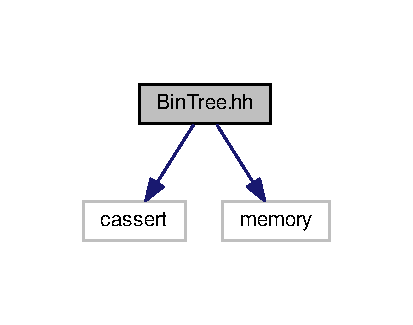
\includegraphics[width=198pt]{_bin_tree_8hh__incl}
\end{center}
\end{figure}
\subsection*{Classes}
\begin{DoxyCompactItemize}
\item 
class \hyperlink{class_bin_tree}{Bin\+Tree$<$ T $>$}
\end{DoxyCompactItemize}

\hypertarget{_experiment_8hh}{}\section{Referència del Fitxer Experiment.\+hh}
\label{_experiment_8hh}\index{Experiment.\+hh@{Experiment.\+hh}}
Inclou el graf de dependències per a Experiment.\+hh\+:
\nopagebreak
\begin{figure}[H]
\begin{center}
\leavevmode
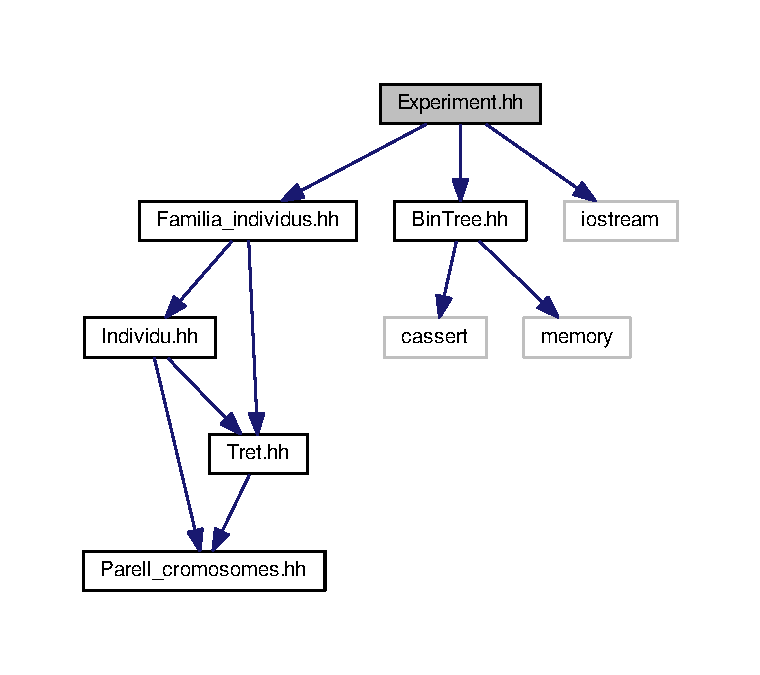
\includegraphics[width=350pt]{_experiment_8hh__incl}
\end{center}
\end{figure}
\subsection*{Classes}
\begin{DoxyCompactItemize}
\item 
class \hyperlink{class_experiment}{Experiment}
\end{DoxyCompactItemize}

\hypertarget{_familia__individus_8hh}{}\section{Referència del Fitxer Familia\+\_\+individus.\+hh}
\label{_familia__individus_8hh}\index{Familia\+\_\+individus.\+hh@{Familia\+\_\+individus.\+hh}}
Inclou el graf de dependències per a Familia\+\_\+individus.\+hh\+:
\nopagebreak
\begin{figure}[H]
\begin{center}
\leavevmode
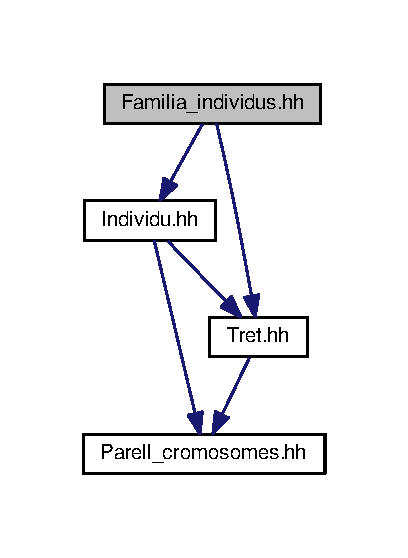
\includegraphics[width=196pt]{_familia__individus_8hh__incl}
\end{center}
\end{figure}
\subsection*{Classes}
\begin{DoxyCompactItemize}
\item 
class \hyperlink{class_familia__individus}{Familia\+\_\+individus}
\end{DoxyCompactItemize}

\hypertarget{_individu_8hh}{}\section{Referència del Fitxer Individu.\+hh}
\label{_individu_8hh}\index{Individu.\+hh@{Individu.\+hh}}
Inclou el graf de dependències per a Individu.\+hh\+:
\nopagebreak
\begin{figure}[H]
\begin{center}
\leavevmode
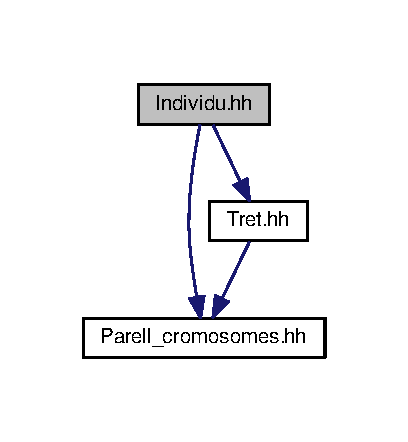
\includegraphics[width=196pt]{_individu_8hh__incl}
\end{center}
\end{figure}
\subsection*{Classes}
\begin{DoxyCompactItemize}
\item 
class \hyperlink{class_individu}{Individu}
\end{DoxyCompactItemize}

\hypertarget{_parell__cromosomes_8hh}{}\section{Referència del Fitxer Parell\+\_\+cromosomes.\+hh}
\label{_parell__cromosomes_8hh}\index{Parell\+\_\+cromosomes.\+hh@{Parell\+\_\+cromosomes.\+hh}}
\subsection*{Classes}
\begin{DoxyCompactItemize}
\item 
class \hyperlink{class_parell__cromosomes}{Parell\+\_\+cromosomes}
\end{DoxyCompactItemize}

\hypertarget{_tret_8hh}{}\section{Referència del Fitxer Tret.\+hh}
\label{_tret_8hh}\index{Tret.\+hh@{Tret.\+hh}}
Inclou el graf de dependències per a Tret.\+hh\+:
\nopagebreak
\begin{figure}[H]
\begin{center}
\leavevmode
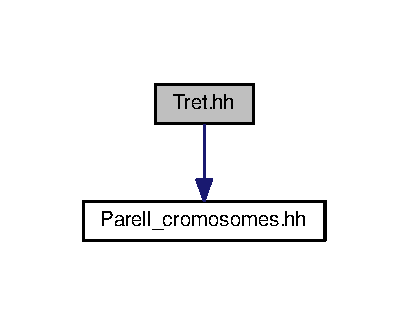
\includegraphics[width=196pt]{_tret_8hh__incl}
\end{center}
\end{figure}
\subsection*{Classes}
\begin{DoxyCompactItemize}
\item 
class \hyperlink{class_tret}{Tret}
\end{DoxyCompactItemize}

%--- End generated contents ---

% Index
\backmatter
\newpage
\phantomsection
\clearemptydoublepage
\addcontentsline{toc}{chapter}{Índex}
\printindex

\end{document}
